\section{Gleichungen {\formelbuch{????}}}
\vspace{.3cm}
	\renewcommand{\arraystretch}{1.2}
	\begin{tabularx}{540pt}{|p{160pt}|p{180pt}|X|}
		\multicolumn{3}{|c|}{}\\[-10mm]
			\hline
			linearer MW & absoluter MW (gleichrichtwert)  & quadratischer MW(Effektivwert) \\
			
			$\dfrac{1}{b-a}\int\limits_a^b f(x)dx$&
			$\dfrac{1}{b-a}\int\limits_a^b |f(x)|dx$&
			$\sqrt{\dfrac{1}{b-a} \int\limits_a^b |f(x)|^2 dx}$\\
			\hline
		
		Tangentengleichung & Normalengleichung  & Hessesche Normalform \\
		
		$y-y_0=m(x-x_0)$ &
		$y-y_0=-\frac{1}{m}(x-x_0)$ &
		$x\cdot \cos\varphi_0 +y\cdot \sin\varphi_0=r_0$ \\
		\hline
		
		Abstand zum Ursprung& Doppelpunkt& glatte Kurve(keine Ecken)\\
		
		$\dfrac{|y_0 - m \cdot x_0|}{\sqrt{m^2 + 1}}$ &
		$t_1 \neq t_2 \Rightarrow P(t_1)=P(t_2)$&
		$\dot{\varphi(t)}^2+\dot{\psi(t)}^2\neq 0$\\
		\hline
		
		Länge Subtangente & Länge Subnormale& \\
		
		$\dfrac{y_0}{|y_0'|}$&
		$|y_0' \cdot y_0|$&
		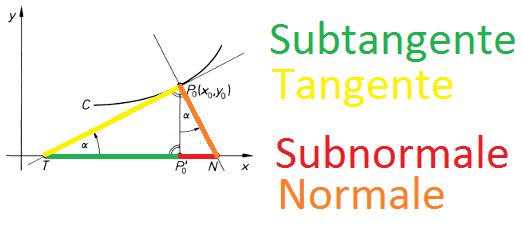
\includegraphics[width = 4cm]{bilder/3_tangent}\\
		\hline
		
		\multicolumn{3}{|c|}{
		\parbox{450pt}{\textbf{Berührung in n-ter Ordnung:} Zwei explizit gegebene Kurven $y = f(x)$ und $y = g(x)$ berühren einander im
		Punkt P $x_0, y_0$ von der Ordnung $n$, wenn die Funktionswerte und die ersten
		$n$ Ableitungen existieren und übereinstimmen.\\
		$f(x_0) = g(x_0);\; f'(x_0) = g'(x_0);\; f''(x_0) = g''(x_0);\;\ldots ;
		\;f^{(n)}(x_0) = g^{(n)}(x_0)\; \qquad f^{(n+1)}(x_0) \neq g^{(n+1)}(x_0)$\\
		Für annäherung von Polynom an beliebige Kurve}}\\
		\hline
	\end{tabularx}
	\renewcommand{\arraystretch}{1}
	
	\subsection{Scheitel \formelbuch{257}} %Seitenzahlen OK 10 Auflage
		Scheitelpunkte sind Extremalwerte der Kr"ummungs- bzw. Kr"ummungsradiusfunktion.
		Falls bei $\kappa'(x)$ an der Stelle $x_0$ ein Vorzeichenwechsel besteht, existiert dort
		eine Extremalstelle. 
	
	\subsection{Kr"ummung \formelbuch{253-255}} %Seitenzahlen OK 10 Auflage
		\begin{tabular}{l|c|r}
			$\kappa > 0 \quad\Rightarrow$ \quad Linkskr"ummung $\iff$ konvex &
			$\kappa = 0 \quad\Rightarrow$ \quad Wendepunkt \quad & \quad
			$\kappa < 0 \quad\Rightarrow$ \quad Rechtskr"ummung $\iff$ konkav
			\\ 
		\end{tabular}
